%% ------------------------------------------------------------------------- %%
\chapter{Tecnologias}
\label{cap:tecnologias}
\section{Ruby on Rails}
\subsection{Ruby}
    \par A criação da linguagem Ruby data de 1995 no Japão por Yukihiro "Matz" Matsumoto sob forte influência de outras linguagens como Perl, SmallTalk, Eiffel, Ada e Lisp e tinha como objetivo equilibrar programação funcional, imperativa e orientação a objetos, segundo o próprio Matz: "Eu queria uma linguagem interpretada que fosse mais poderosa do que Perl e mais orientada à objetos do que Python2.". (\cite{rubydocs}
\begin{itemize}
\item{Flexibilidade:}
    \par Ruby cresceu devido a sua grande flexibilidade sendo possível alterar, remover ou acrescentar partes da linguagem à vontade, imagine o seguinte exemplo: um usuário prefere utilizar a palavra plus ao invés do operador matemático(  +  ), ele poderia então adicionar esse método à classe nativa do Ruby Numeric pois em ruby os operadores matemáticos são considerados açúcares sintáticos.
\\Exemplo:
\begin{lstlisting}[frame=single]
class Numeric
          def plus(x)
                self.+(x)
          end
    end

    y = 5.plus 6
    # y agora eh igual a 11
\end{lstlisting}
\item{Closures:}
    \par Em ruby o closures são chamadas de blocos e são funções que podem ser tratadas como uma variável isso quer dizer que podem ser passadas como argumentos de métodos, serem atribuidas a outras variáveis, etc.
    \par As \emph{closures} armazenam os valores das variáveis que estavam no escopo quando a função foi definida e são capazes de acessar tais variáveis mesmo que sejam executadas em um escopo diferente. \footnote{Fonte: Site Point \url{https://www.sitepoint.com/closures-ruby/}}
\\
Exemplo:
\begin{lstlisting}[frame=single]
search_engines =
  %w[Google Yahoo MSN].map do |engine|
    "http://www." + engine.downcase + ".com"
  end
\end{lstlisting}
\item{Módulos:}
    \par Diferente de outras linguagens orientadas a objetos o Ruby suporta apenas herança simples porém de forma proposital.  Em ruby existe o conceito de módulos que são coleções de métodos que podem ser adicionadas à uma classe por meio de um mixin.
    As classes podem fazer o mixin de um método e receber todos os métodos dele diretamente.
Exemplo:
\begin{lstlisting}[frame=single]
class MyArray
          include Enumerable
    end
\end{lstlisting}

\end{itemize}
\subsection{Rails}

\par David Heinemeier Hansson extraiu o Ruby on Rails do seu próprio trabalho realizado na empresa Basecamp e foi lançado de maneira open-source pela primeira vez em 2004, inicialmente ele estava desenvolvendo seu projeto utilizando PHP porém apesar de conseguir desenvolver de maneira bastante ágil a repetição de código incomodava-o. \
\par Rails é um framework web escrito em Ruby implementado seguindo o padrão MVC totalmente \emph{server-side} sendo considerado portanto um \emph{framework back-end}.
\par Rails oferece uma estrutura para banco de dados, \emph{web service} e \emph{web pages} além de encorajar padrões de engenharia de software já consagrados ( \cite{railswiki} tais como:
\begin{itemize}
\item {\emph{Convention over Configuration} (CoC):}
    \par Apesar de algumas críticas por adicionar obscuridade pois não existe uma forma clara de verificar o comportamento esperado ruby adota alguns padrões de configuração visando padronizar o código e tirar do desenvolvedor a decisão de como usar o arcabouço sem que isso tire sua flexibilidade. Por exemplo se existir um objeto chamado User então sua tabela por convenção se chamará users e correspondente \emph{controller} será UsersController ( no plural) pois esse é padrão definido para o framework e de outra forma o seu controller ou database não estaria associado ao modelo User, a menos que você mudasse as configurações para não utilizar as convenções padrão.

\item {\emph{Don't Repeat yourself} (DRY):}

    \par Visando diminuir a repetição de informações de qualquer tipo em rails frequentemente ao utilizar o comportamento padrão da linguagem o desenvolvedor terá a impressão de que tal comportamento não tem sem explicação já que sua implementação está escondida dentro do código do próprio Rails porém evitando que dessa forma o programador tenha que reescrever várias vezes um mesmo código para determinado comportamento. \footnote{Fonte: Wikipedia \url{https://en.wikipedia.org/wiki/Don\%27t_repeat_yourself}}

\item { \emph{Active Record Pattern}:}
    \par O padrão Active Record sugere uma interface específica para acessar objetos em um banco de dados relacional contendo funções tais como INSERT, UPDATE, DELETE, etc.
    \par Uma tabela ou \emph{view} será associada a uma classe então uma instância de objeto estará associada a uma única entrada na respectiva tabela.
    \par Em Rails a biblioteca ActiveRecord implementa o padrão ORM e além disso acrescenta herança e associações resolvendo dois problemas substanciais do padrão.
    \par ActiveRecord é o "model" padrão do componente MVC porém é possível trocá-lo por outra implementação do framework Rails caso o desenvolvedor prefira.
\end{itemize}
    \par Em um sentido mais amplo Rails é mais que uma biblioteca de Software ou API: é um projeto central de uma vasta comunidade que produz plugins para facilitar e construir projetos complexos de web site. Foi graças a essa comunidade que compartilham ferramentas e contribuem para o projeto Rails criando bibliotecas open source ( chamadas de Ruby Gems ou apenas Gems \footnote{Fonte: Wikipedia \url{https://en.wikipedia.org/wiki/RubyGems}}) que o o uso de rails tem crescido de forma significante nos últimos anos ganhando fama entre startups devido a sua  facilidade e desevolvimento que permite criar sistemas complexos e testar idéias rapidamente.

\section{Heroku}
\par Heroku é uma Paas implementada utilizando \emph{cloud computing} criada em 2007 utilizada como um modelo de \emph{Deployment} para Aplicações Web. ( \cite{herokuwiki})
\par A rede do Heroku roda os aplicativos em containers virtuais que executam um ambiente de execução confiável. Esses containers são chamados de Dynos e podem rodar códigos escritos em Nodejs, Ruby, PHP, Go, Scala, Python, Java, Clojure.
\par O \emph{deploy} de uma aplicação no Heroku é bastante simples o que contribuiu para sua popularização principalmente entre startups que necessitam de agilidade para subir novas atualizações.
\par A aplicação é enviada para o Heroku por meio de uma conexão direta via GitHub, Dropbox ou alguma API.
\par Enviado o código-fonte ele então é convertido em uma aplicação interpretando as dependências de outras bibliotecas seguindo o padrão de cada linguagem. No caso do USP Eventos que foi feito utilizando Ruby as dependências ficam armazenadas no próprio Gemfile da aplicação.
\par Feito o upload da aplicação um container com uma virtualização de Unix é disponibilizado, o Dyno da aplicação. Tal container é pre-carregado com algumas configurações prévias da aplicação: um nome gerado automaticamente, variáveis de ambiente e \emph{add-ons} se existirem.
\par O Heroku então inicializa o Dyno com a aplicação, carrega-a e então realiza o \emph{deploy} da mesma.
\par Através do DNS Server oferecido pelo próprio Heroku a aplicação fica acessível por meio de um domínio na forma <nome da aplicação>.herokuapp.com sendo possível redirecionar seu domínio particular para refletir o DNS disponibilizado.
\section{Travis CI}
\par Travis CI é um serviço de integração contínua usado para testar projetos hospedados no Github.
\par Toda vez que um commit para o repositório selecionado no Gitbhub o Travis irá executar as diretrizes especificadas no arquivo travis.yml que contém os comandos necessários para rodar os testes automatizados da aplicação, como é o caso do USP Eventos (figura \ref{fig:travis}).
\begin{figure}[htb]
\centering
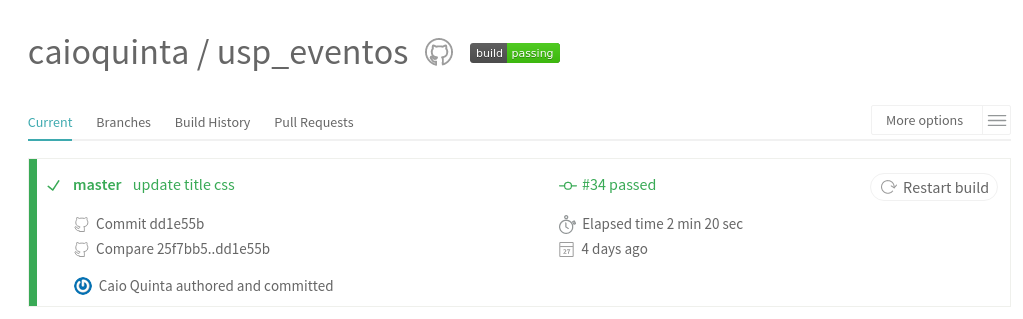
\includegraphics[width=15cm]{figuras/travis}
\caption{\label{fig:travis} O repositório USP Eventos no Travis CI.}
\end{figure}

\section{Trello}
\par Trello é um gerenciador de projetos online desenvolvido pela Fog Creek Software lançado em 2011.
\par Possui uma interface amigávelna qual é possível criar tarefas e colunas conforme as preferências do usuário sendo bastante utilizado em conjunto com uma abordagem kanbam para gerenciamento.

\section{Google Analytics e Google Tag Manager}
TODO
\section{Painel de opiniões Populares - POP}
\par Com o intuito de definir o interesse do público alvo por meio de uma enquete colaborativa utilizamos o POP como sistema de votação devido a sua propriedade interativa na qual os usuários poderiam adicionar itens à enquete principal.
\par Desenvolvido por estudantes do próprio IME dentro da disciplina de Laboratório de Programação Extrema à pedido da INDX o POP é uma plataforma de pesquisa de opinião pública que possui o objetivo de realizar enquetes nas quais os próprios usuários possam interagir e criar novas opções com o intuti de medir quais são as prioridades de projetos para a região.
\par Foi permitida a utilização da plataforma implementada em uma instância separada com o nome de POP-TCC. para realização da enquete junto à comunidade USP para definir qual seria o tema do projeto.
\par Foi feita uma modificação no sistema POP original para o POP-TCC na qual os usuários só poderiam votar de maneira positiva nas enquete ao contrário do sistema original que permitia votos negativos e até ocultamento dos itens da enquete que fossem muito negativados pelos usuários.

\section{HeatMap}
\par O serviço fornecido pela plataforma Heatmap.me consiste em prover uma api que é capaz de capturar os cliques em uma determinada página e mostrá-los na forma de uma mapa de calor.
\par Um mapa de calor é uma representação gráfica dos cliques em uma página na qual conforme uma determinada região for recendo mais cliques sua cor é alterada (figura \ref{fig:heatmap_explanation}).
\begin{figure}[htb]
\centering
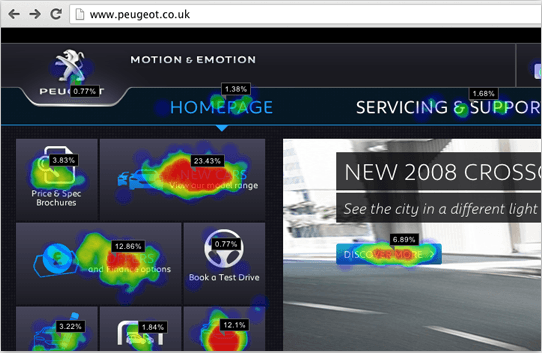
\includegraphics[width=15cm]{figuras/heatmap_explanation}
\caption{\label{fig:heatmap_explanation} O repositório USP Eventos no Travis CI.}
\end{figure}
\par Sendo que as cores inicialmente começam em um tom verde quando foram clicadas poucas vezes sendo gradativamente alteradas para cores mais "quentes" tais como laranja ou vermelho conforme os cliques na mesma região são feitos.